%"runningheads" enables:
%  - page number on page 2 onwards
%  - title/authors on even/odd pages
%This is good for other readers to enable proper archiving among other papers and pointing to content.
%Even if the title page states the title, when printed and stored in a folder, when blindly opening the folder, one could hit not the title page, but an arbitrary page. Therefore, it is good to have title printed on the pages, too.
\documentclass[runningheads,a4paper]{llncs}

% use subpackage
\usepackage{subfigure}

% tikz package
\usepackage{tikz}
\usetikzlibrary{shapes.geometric, arrows}

%Even though `american`, `english` and `USenglish` are synonyms for babel package (according to https://tex.stackexchange.com/questions/12775/babel-english-american-usenglish), the llncs document class is prepared to avoid the overriding of certain names (such as "Abstract." -> "Abstract" or "Fig." -> "Figure") when using `english`, but not when using the other 2.
\usepackage[english]{babel}

%better font, similar to the default springer font
%cfr-lm is preferred over lmodern. Reasoning at http://tex.stackexchange.com/a/247543/9075
\usepackage[%
rm={oldstyle=false,proportional=true},%
sf={oldstyle=false,proportional=true},%
tt={oldstyle=false,proportional=true,variable=true},%
qt=false%
]{cfr-lm}
%
%if more space is needed, exchange cfr-lm by mathptmx
%\usepackage{mathptmx}

\usepackage{graphicx}

%extended enumerate, such as \begin{compactenum}
\usepackage{paralist}

%Sorts the citations in the brackets
%It also allows \cite{refa, refb}. Otherwise, the document does not compile.
%  Error message: "White space in argument"
\usepackage{cite}

\usepackage[T1]{fontenc}

%for demonstration purposes only
\usepackage[math]{blindtext}

%for easy quotations: \enquote{text}
\usepackage{csquotes}

%enable margin kerning
\usepackage{microtype}

%tweak \url{...}
\usepackage{url}
\urlstyle{same}
%improve wrapping of URLs - hint by http://tex.stackexchange.com/a/10419/9075
\makeatletter
\g@addto@macro{\UrlBreaks}{\UrlOrds}
\makeatother
%nicer // - solution by http://tex.stackexchange.com/a/98470/9075
%DO NOT ACTIVATE -> prevents line breaks
%\makeatletter
%\def\Url@twoslashes{\mathchar`\/\@ifnextchar/{\kern-.2em}{}}
%\g@addto@macro\UrlSpecials{\do\/{\Url@twoslashes}}
%\makeatother

%required for pdfcomment later
\usepackage{xcolor}

% new packages BEFORE hyperref
% See also http://tex.stackexchange.com/questions/1863/which-packages-should-be-loaded-after-hyperref-instead-of-before

%enable hyperref without colors and without bookmarks
\usepackage[
%pdfauthor={},
%pdfsubject={},
%pdftitle={},
%pdfkeywords={},
bookmarks=false,
breaklinks=true,
colorlinks=true,
linkcolor=black,
citecolor=black,
urlcolor=black,
%pdfstartpage=19,
pdfpagelayout=SinglePage,
pdfstartview=Fit
]{hyperref}
%enables correct jumping to figures when referencing
\usepackage[all]{hypcap}

%enable nice comments
\usepackage{pdfcomment}
\newcommand{\commentontext}[2]{\colorbox{yellow!60}{#1}\pdfcomment[color={0.234 0.867 0.211},hoffset=-6pt,voffset=10pt,opacity=0.5]{#2}}
\newcommand{\commentatside}[1]{\pdfcomment[color={0.045 0.278 0.643},icon=Note]{#1}}

%compatibality with TODO package
\newcommand{\todo}[1]{\commentatside{#1}}

%enable \cref{...} and \Cref{...} instead of \ref: Type of reference included in the link
\usepackage[capitalise,nameinlink]{cleveref}
%Nice formats for \cref
\crefname{section}{Sect.}{Sect.}
\Crefname{section}{Section}{Sections}

\usepackage{xspace}
%\newcommand{\eg}{e.\,g.\xspace}
%\newcommand{\ie}{i.\,e.\xspace}
\newcommand{\eg}{e.\,g.,\ }
\newcommand{\ie}{i.\,e.,\ }

%introduce \powerset - hint by http://matheplanet.com/matheplanet/nuke/html/viewtopic.php?topic=136492&post_id=997377
\DeclareFontFamily{U}{MnSymbolC}{}
\DeclareSymbolFont{MnSyC}{U}{MnSymbolC}{m}{n}
\DeclareFontShape{U}{MnSymbolC}{m}{n}{
    <-6>  MnSymbolC5
   <6-7>  MnSymbolC6
   <7-8>  MnSymbolC7
   <8-9>  MnSymbolC8
   <9-10> MnSymbolC9
  <10-12> MnSymbolC10
  <12->   MnSymbolC12%
}{}
\DeclareMathSymbol{\powerset}{\mathord}{MnSyC}{180}

% correct bad hyphenation here
\hyphenation{op-tical net-works semi-conduc-tor}

\begin{document}

%Works on MiKTeX only
%hint by http://goemonx.blogspot.de/2012/01/pdflatex-ligaturen-und-copynpaste.html
%also http://tex.stackexchange.com/questions/4397/make-ligatures-in-linux-libertine-copyable-and-searchable
%This allows a copy'n'paste of the text from the paper
\input glyphtounicode.tex
\pdfgentounicode=1

\title{iParking -- Real-Time Parking Space Monitor and Guiding System with Cloud Service}
%If Title is too long, use \titlerunning
%\titlerunning{Short Title}
\titlerunning{iParking}

%Single insitute
\author{Ching-Fei Yang \and You-Huei Ju \and Chung-Ying Hsieh \and
Chia-Ying Lin \and \\ Meng-Hsun Tsai \and Hui-Ling Chang}
%If there are too many authors, use \authorrunning
\authorrunning{Ching-Fei Yang et al.}
\institute{
	Department of Computer Science and Information Engineering,\\ 
	National Cheng Kung University,\\
	\email{e84016184@mail.ncku.edu.tw}
}

\maketitle

\begin{abstract}
By the popularization of cars, average number of vehicles owned by one person
grows with passing days. However, the number of parking areas is out of
proportion. In order to satisfy the requirements of parking space and
reduce illegal parking, we propose iParking, a real-time parking space
monitoring and guiding system, in this paper. 
We lay emphasis on roadside parking. The system determines and records
empty parking spaces through cloud computing, wireless technology
between vehicles, and image analysis. It tells you the nearest location
of empty parking space while drivers have requests. We expect the system
to cause attention to more people and government while it solves relative
problems about parking space. 
\end{abstract}

\keywords{cloud computing, image recognition, parking space management, wireless technology}

%%%%%%%%%%%%%%%%%%%%%%%%%%%%%%%%%%%%%%%%%%%%%%%%%%%%%%%%%%%%%%%%%%%%%%%%%%%%%%%
\section{Introduction}\label{sec:intro}
%%%%%%%%%%%%%%%%%%%%%%%%%%%%%%%%%%%%%%%%%%%%%%%%%%%%%%%%%%%%%%%%%%%%%%%%%%%%%%%

Recently, parking problem has become people's harassment. 
It is shown from statistical data in Ministry of
Transportation, Taiwan that the number of registered vehicles is
7,554,319 until December 2014 \cite{motc}; However, it is also mentioned that
the number of legal parking space is about four million in total. 
Furthermore, it will cause several problems such as the extremely slow
speed while finding parking space, scrambling for roads with scooters,
parking temporarily in dangerous part, or driving U-turn illegally. The
behavior will not only break the safety and regular of transportation
but also make noise and consume resource. 
It is easy to observe that some vehicles need to find parking space by
themselves while roadside parking spaces are not enough. The situation
will bring out arbitrary parking, and it is also the main reason of
illegal parking. 

Over the last few years, LBS (Location-Based Service) \cite{LBS} is getting noticed along with
the appearance of smartphones. LBS can apply broadly to different area
like health, job, daily life, and etc. Thus, how to use LBS to help
different users find the appropriate parking space is vital. The usage
of monitoring parking space now is to provide roadside parking space's
locations at best, but it will not tell drivers where the vacant space
is. Thus, we would like to develop a monitor and guiding system focus on
roadside parking to provide the information of nearby parking space and
help drivers park with the fastest way.

We will introduce the system in four parts. First of all, know what is
the demand of our work and compare with other techniques. Next, show the
details, especially features and structure of our service. In addition,
demonstrate how we implement and design the system. Finally, make a
conclusion, discuss more about future work.


%%%%%%%%%%%%%%%%%%%%%%%%%%%%%%%%%%%%%%%%%%%%%%%%%%%%%%%%%%%%%%%%%%%%%%%%%%%%%%%
\section{Related Work}\label{sec:relatedWork}
%%%%%%%%%%%%%%%%%%%%%%%%%%%%%%%%%%%%%%%%%%%%%%%%%%%%%%%%%%%%%%%%%%%%%%%%%%%%%%%

%
\subsection{Demand of parking space}
%

In the statistical table of important indicators from Ministry of
Transportation, Taiwan \cite{motc}, it is pointed out that parking space is one
of the important indicators in addition to the number of vehicles.
\Cref{fig:StatisticalTable} is the comparison chart between the number of vehicles and
parking spaces from 2006 to 2014 in Taiwan.

\begin{figure}[tbp]
\begin{center}
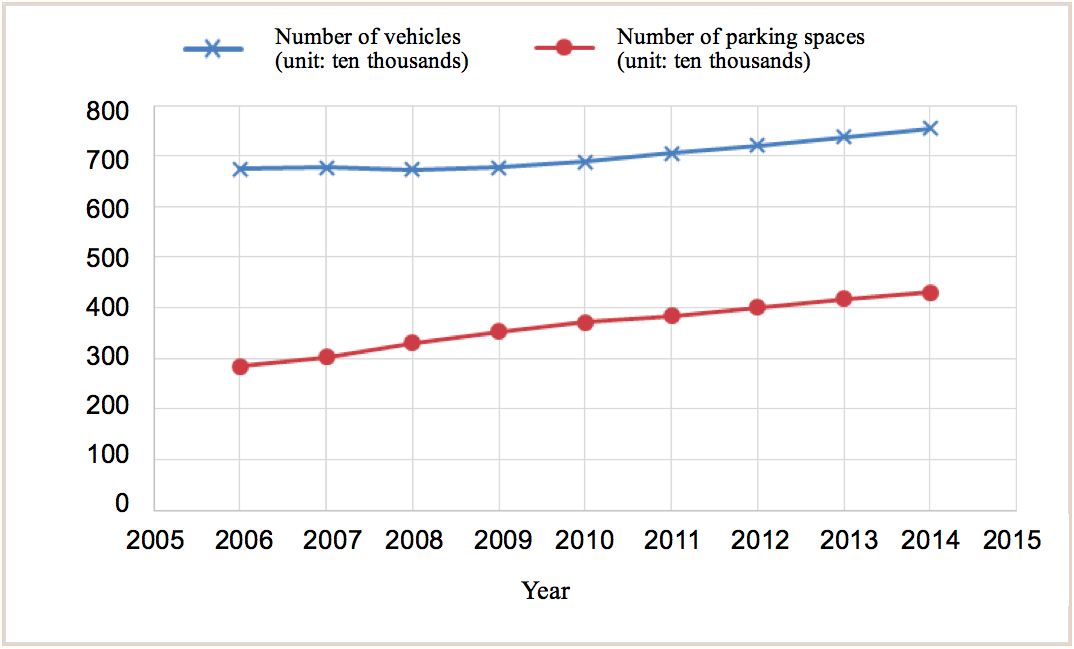
\includegraphics[width=0.8\textwidth]{Figures/Statistical_Table.png}
\end{center}
\caption{Statistical table of vehicles and parking spaces' number from
2006 to 2014}
\label{fig:StatisticalTable}
\end{figure}

It is shown from \Cref{fig:StatisticalTable} that the difference between supply and demand
of parking space is about two million. In addition, it is pointed out
from trend of line that the growth rate of vehicles and parking spaces
is closed. However, it is not simple to add parking spaces because it
involves road network planning. In this knotty situation, it becomes
vital and urgent to solve the management of parking space in order to
make good use of limited resource.

Furthermore, some recent researches verify that people would rather
spend more time finding roadside parking space than off-street parking
even if there are vacant spaces in the off-street parking lot \cite{OnStreetParking}. Take
Tainan City for example, service in parking lot does not meet drivers'
expect, such as high parking fee, mess surroundings, or etc. Hence, the
situation results in low usage rate of parking lot and shortage of
roadside parking space. Thus, to solve the problem of roadside parking
is necessary.

%
\subsection{Existing parking space monitored technique}
%

All of existing parking space monitored techniques are limited to
parking lot and only supported by sensors. For instance, intelligent
parking lot uses wireless sensor network, ZIBEE, pressure sensors
\cite{PaymentSystem, IOV2015}.
They update database by sensors to know if it is empty. The another
instance is Eco-Community plan developed by several schools
\cite{EcoCommunity}. Its
main method is using the sensitivity of the sensor, Octopus II,
updating changes to database. Therefore, the changes will tell users
information about parking spaces. However, the two techniques have a big
constraint when it comes to downtown area. It is a huge challenge to set
up sensors for all parking spaces in downtown due to the fee of building
and maintenance. That is to say, both of them are not suitable to
roadside parking in comparison with our system.

As regards other apps in the market, they are connected to nearby
parking lot, offering real-time information. However, only few of
them mention payment information about roadside parking. In conclusion,
none of the apps in the market provide function to find roadside parking
spaces until now.

%%%%%%%%%%%%%%%%%%%%%%%%%%%%%%%%%%%%%%%%%%%%%%%%%%%%%%%%%%%%%%%%%%%%%%%%%%%%%%%
\section{Service and System Structure}\label{sec:service}
%%%%%%%%%%%%%%%%%%%%%%%%%%%%%%%%%%%%%%%%%%%%%%%%%%%%%%%%%%%%%%%%%%%%%%%%%%%%%%%

%
\subsection{Software platform}
%

We choose smartphone and related device to complete mobility, driving
recorder, and Network communication by reason of the target users,
people with mobile vehicle. We build the application base on Android,
using Java to implement code structure and GUI design.

%
\subsection{Features}
%

%
\subsubsection{Cloud storage and computing}
%

Cloud Storage is an online service which can save data on virtual server
through Internet. The service become more and more popular due to the
popularity of Internet and the increasing demand of data storage. That
is to say, simply save data in actual hard dick is getting insufficient.
Therefore, limited storage devices will bring more benefit by Internet
and storage virtualization technique.

In order to improve the efficiency of driving records, and reduce the
capacity of mobile device. We will refer to existing cloud storage
service, analyzing data through servers in cloud, and send the parking
information to users who have request.

%
\subsubsection{Static image streaming}
%

Streaming media is a process to compress a series of media data, send
through network section, and offer real-time media service on the
Internet. By the technique, media data are able to watch without
downloading whole media. Therefore, it is called ``streaming'' because
data in the process behaves like running water.

We can say that static image streaming is to connect images,
record the event over the next period of time. Under the premise that
analyzing driving records accurately, we will use static image streaming
to lessen the burden instead of sending whole driving record.

%
\subsubsection{Analyzing vacant parking space}
%

In the reference \cite{ParkingSpot}, the author has proposed solutions to detect if
parking spaces are vacant. Its technique includes Hough line detection
and Canny edge detection, implementing by OpenCV library. The
original method has two limitations. The first one is that it can only
identify one photo at a time while the another is that only the parking
space at bottom right corner can be identified. We breakthrough them by
using static image streaming.


%
\subsection{Efficacy}
%

%
\subsubsection{Monitoring parking space}
%

The situation of parking space is different from area, timing, and
location. Therefore, the key point is how to monitor the specific
parking space immediately. Besides, if there are many people use this
service at the same time, it will be fairly accurate with steadily
update.

%
\subsubsection{Saving and analyzing driving recorder}
%

In the process of detecting vacant parking space's condition, it is
necessary to analyze big data and use large storage. Hence, we use cloud
service and client-server model to handle and send all the requests in
order to reduce the usage of memory, storage, and workload.

%
\subsubsection{Data transmission}
%

If the goal is to keep high accuracy and immediacy, the system will
bring out high Internet usage because it continuing transfers driving
recorder. Therefore, we will capture driving image with a fixed distance
according to speed of the vehicle. Coordinating with GPS position, it
will become image streaming instead of video. That is to say, capacity
and the time of data transmission can be saved.

%
\subsection{Structure}
%

We mainly focus on car owners. Besides, we will use our own approach to
detect driving record automatically and communicate between vehicles.
The application is built on Android, expected to run the program on
driving recorders. We will limit to a specific road section while
testing and developing the system.

Four steps are supposed to proceed. First, determine the specific road
section, and collect data; Next, sort out the collected data. Start
to plan the structure of program; Then, begin to develop the program,
add GUI, do simulation, and test system. Finally, analyze and present
whole the research. \Cref{fig:flowDiagram} is the flow diagram of these steps.

\begin{figure}[tbp]
\begin{center}
	% Define block styles
	\tikzstyle{startstop} = [rectangle, rounded corners, minimum
width=3cm, minimum height=1cm,text centered, text width=3cm, draw=black, fill=red!30]
	\tikzstyle{process} = [rectangle, minimum width=3cm, minimum
height=1cm, text centered, text width=3cm, draw=black, fill=orange!30]
	\tikzstyle{decision} = [diamond, minimum width=3cm, minimum height=1cm,
text centered, text width=3cm, draw=black, fill=green!30]
	\tikzstyle{arrow} = [thick,->,>=stealth]
	\tikzstyle{io} = [trapezium, trapezium left angle=70, trapezium
right angle=110, minimum width=2cm, minimum height=1cm, text centered,
text width=3cm,  draw=black, fill=blue!30]
	    
	\begin{tikzpicture}[node distance=2cm]
	    % Place nodes
	    \node [startstop] (init) {initialize model};
	    \node [process, below of=init] (function) {plan for each function};
	    \node [process, below of=function] (space) {provide space to store driving record};
	    \node [io, below of=space] (receive) {receive users' requests};
	    \node [process, right of=receive, xshift=2cm] (design) {design UI interface};
	    \node [process, above of=design] (system) {implement the whole system};
	    \node [decision, above of=system, yshift=1.5cm] (testing) {test client and server side separately};
	    \node [decision, right of=testing, xshift=3cm] (integrate) {integrate all structures};
		\node [startstop, below of=integrate, yshift=-1.5cm] (end) {stop};
	    % Draw edges
	    \draw [arrow] (init) -- (function);
	    \draw [arrow] (function) -- (space);
	    \draw [arrow] (space) -- (receive);
		\draw [arrow] (receive) -- (design);
		\draw [arrow] (design) -- (system);
		\draw [arrow] (system.110) -- (testing.-96);
	    \draw [arrow] (testing) -- node [anchor=north] {yes} (integrate);
	    \draw [arrow] (testing.-85) -- node [anchor=west] {no}(system.70);
	    \draw [arrow] (integrate) -- node [anchor=west] {yes} (end);
	    \draw [arrow] (integrate) -- node [anchor=north] {no}(system);
	\end{tikzpicture}
\end{center}
\caption{Research flow diagram}
\label{fig:flowDiagram}
\end{figure}

%
\subsubsection{Building cloud service and algorithm design}
%

The main usage of cloud service is to implement each operated function,
handle users' request, and provide storage to save driving records. The
operated function includes receiving image data from users, analyzing
images, building database, searching database, and etc. Hold time is the
first concern because of massive calculation. The other factor is the
availability of data, for example, we will not use old data and data
which has been analyzed in the same location. This algorithm will help
reduce repeated operations, furthermore, it helps us make sure that we
are analyzing real-time image in every data.

%
\subsubsection{Program structure in device and UI design}
%

We will plan our service with relation to different characters. For
example, it is necessary for users to search nearby parking space, it is
required for devices to send image information to servers in cloud, and it
is important for servers to analyze and collect data. As for UI design
in app, in order to realize convenient searching function and interface,
it need to be designed from the view of users.

The error of GPS measurement is about 5 to 10 meters. We can say
that it is about 1 or 2 roadside parking spaces. In order to enhance the
accuracy, we will combine Google Maps API, take the advantage of its
navigation and distance matrix service. Besides accessing the speed and
distance of vehicles, the API can also help send GPS location to keep
loading and operating fast in the device.

When it comes to clients, we will check whether there is anyone else
sending the same information of specific location at the same time or
not. It will not send information if anyone else is sending the data.
However, if there is not anyone else sending the data, we plan to
capture image immediately after moving a small and appropriate distance
before sending to servers in cloud.

\begin{figure}[tbp]
	\centering
		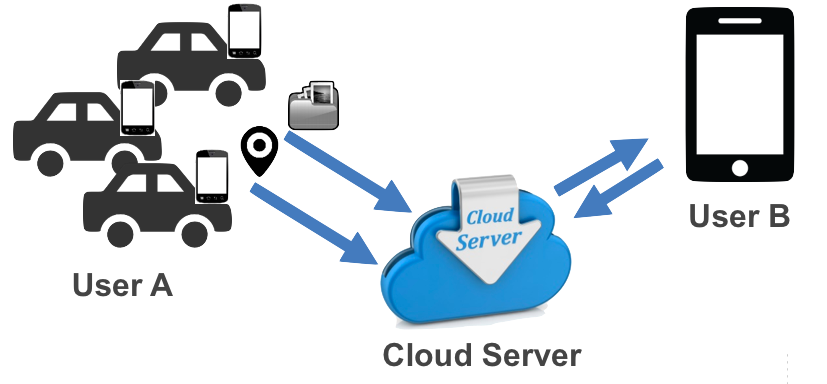
\includegraphics[width=0.8\textwidth]{Figures/flowChart.png}
		\caption{System flow chart}
		\label{fig:system}
\end{figure}


%%%%%%%%%%%%%%%%%%%%%%%%%%%%%%%%%%%%%%%%%%%%%%%%%%%%%%%%%%%%%%%%%%%%%%%%%%%%%%%
\section{Implementation}\label{sec:implementation}
%%%%%%%%%%%%%%%%%%%%%%%%%%%%%%%%%%%%%%%%%%%%%%%%%%%%%%%%%%%%%%%%%%%%%%%%%%%%%%%

The system is divided into three parts - image recongization, cloud
server, and client's application. At first, the three parts will be implemented
separately. They will be combined and operate after they all make a certain proportain.

\subsection{Image recognition of roadside parking space}

Image recognition and analysis of roadside parking space is implemented by C++ with
OpenCV library. The program will return if the image of parking space is
vacant after received an image.

\subsubsection{Setting ROI (Region of Interest)}

First, the program will convert the image into gray scale. The reason is
that the perspective of image will affect the degree of image
recognition. Moreover, the image will be divided into four equal parts.
Only the right-bottom part will be reserved because the spaces are
usually located in the right hand side.

\begin{figure}[tbp]
	\subfigure[Gray scale image] {
		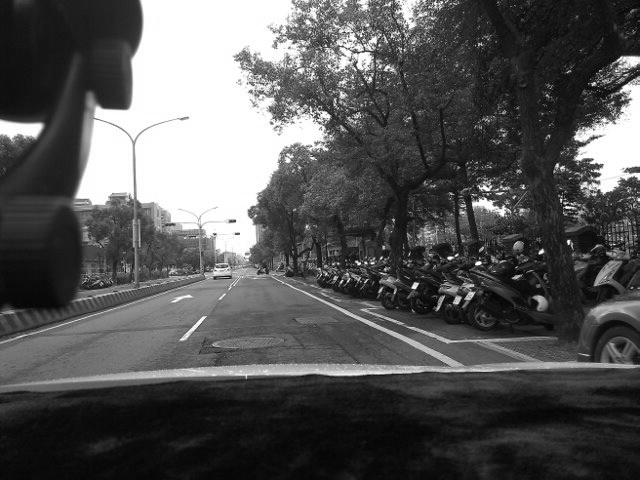
\includegraphics[scale=0.8]{Figures/grayScaleImage.png}
	}
	\hspace{0.2in}
	\subfigure[ROI image] {
		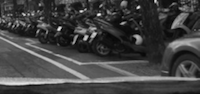
\includegraphics[scale=0.8]{Figures/ROIImage.png}
	}
	\caption{Setting ROI}
	\label{fig:ROI}
\end{figure}

\subsubsection{Sides detection and Noise reduction on Image} 

The program uses Canny edge detection in OpenCV to find each side of
parking space. Afterward it reduces noise by the way, Median Blur.
(\Cref{sideDetecting})

\begin{figure}[tbp]
	\begin{minipage}{.4\textwidth}
		\centering
		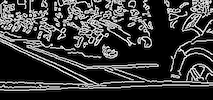
\includegraphics[scale=0.7]{Figures/sideDetecting.png}
		\caption{Detect each side}
		\label{sideDetecting}
	\end{minipage}
	\hspace{0.5in}
	\begin{minipage}{.4\textwidth}
		\centering
		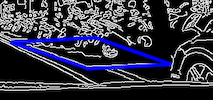
\includegraphics[scale=0.7]{Figures/drawParkingSpace.png}
		\caption{Draw parking space}
		\label{drawParkingSpace}
	\end{minipage}
\end{figure}

\subsubsection{Find out parking spaces}

First, find out straight line with Hough line detection. Detect
which one is the line of parking space by angle and intersection of
lines. (\Cref{drawParkingSpace})

If the appropriate space is not found, the program will return the
result of no vacant space (equals to occupied by vehicle). However, if
the space is found, it will continue to next to detect if the space is
able to use.

\subsubsection{Detect if the parking space is able to use}

If the ratio between the side of parking space and its shelter is more
than a certain number, it means that the space has been occupied.
Therefore, the program will return no vacant spaces. On the contrary, 
it will return there is a vacant parking space.

\begin{figure}[tbp]
	\subfigure[Available parking space] {
		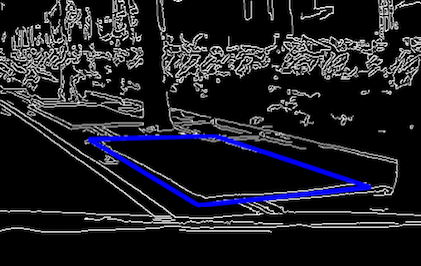
\includegraphics[scale=0.7]{Figures/availableParkingSpace.png}
	}
	\hspace{0.5in}
	\subfigure[Unavailable parking space] {
		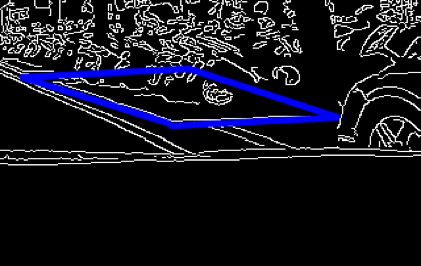
\includegraphics[scale=0.7]{Figures/unavailableParkingSpace.png}
	}
	\caption{Detect parking space}
	\label{detectingParkingspace}
\end{figure}

\subsection{Cloud analyzing server}

After passing image recognition of roadside parking space testing, the
program mentioned above will be moved to cloud service. Moreover, it will
coordinate with the open data offered by government. The data will
provide the information about roadside parking space. Therefore, we are
able to know which road sections do not have spaces, prevent analyze the
images from those sections. We implement the server by nodejs action
hero framework; In addition to offering API with http, we will provide
interface for webpages in order to let users find parking spaces
directly. Non-relational database, Mongo, is also used to accelerate
access and operated speed. 

Servers in cloud will translate longitude and latitude into address
information while receiving GPS information and images by users. Next,
it will compare the road section with open data to confirm if the
section provides parking spaces. After successful analysis, the result
with address will update to database for other users.

\subsection{Mobile APP (client side)}

It is divided into several steps to implement, mainly separated into
user (device) and server side. First, we use Android platform with
Android Studio and Android SDK, which are based on JAVA, to develop
client's application.


\begin{figure}[tbp]
	\subfigure[Home] {
		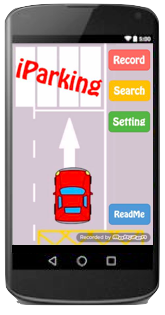
\includegraphics[scale=0.3]{Figures/userHome.png}
		\label{fig:userHome}
	}
	\hspace{0.1in}
	\subfigure[Record] {
		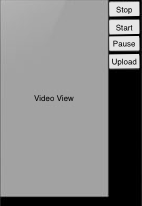
\includegraphics[scale=0.3]{Figures/userRecord.png}
		\label{fig:userRecord}
	}
	\hspace{0.1in}
	\subfigure[Setting] {
		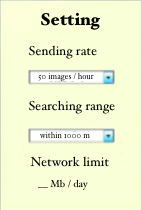
\includegraphics[scale=0.3]{Figures/userSetting.png}
		\label{fig:userSetting}
	}
	\hspace{0.1in}
	\subfigure[Result] {
		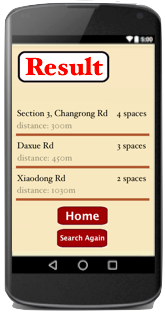
\includegraphics[scale=0.3]{Figures/userResult.png}
		\label{fig:userResult}
	}
	\hspace{0.1in}
	\subfigure[Map] {
		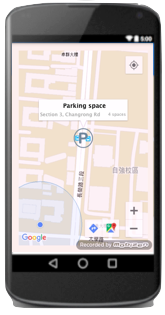
\includegraphics[scale=0.3]{Figures/userMap.png}
		\label{fig:userMap}
	}
	\caption{User interface}
	\label{fig:userInterface}
\end{figure}

\Cref{fig:userInterface} is our main interface and function.
\Cref{fig:userHome} is the first screen of the system. You
can choose the function of both recording and searching.
\Cref{fig:userRecord} is recording screen. It will use device's
camera automatically, temporarily save the records in iParking
folder. The purpose is to let users check the
record, choose if they want to provide it to other users or delete it. After
uploading the record, it will be deleted. \Cref{fig:userSetting}
is the setting page. Users can change their sending rate (network flow)
and searching range while finding parking space.
\Cref{fig:userResult} is the result of searching. Users will know 
how many parking spaces nearby. After choosing the one user prefers, 
the location will be shown on the map like \Cref{fig:userMap}.
Therefore, user can be navigated to the space combined with Google API.

\subsection{Testing}

In the part of testing, we will initially test client and server side
separately, merge them with UI design. Finally, we will test
the integrated system by the following steps. First, a single vehicle.
That is to test with different speed, make sure that static image
streaming is worked with cloud service. Next, test the efficiency of
multiple vehicles. Verify that no images will be in the same
location at the same time. The last step is to confirm that client side
can get the correct information immediately.

%%%%%%%%%%%%%%%%%%%%%%%%%%%%%%%%%%%%%%%%%%%%%%%%%%%%%%%%%%%%%%%%%%%%%%%%%%%%%%%
\section{Conclusion and Future Work}\label{sec:conclusion}
%%%%%%%%%%%%%%%%%%%%%%%%%%%%%%%%%%%%%%%%%%%%%%%%%%%%%%%%%%%%%%%%%%%%%%%%%%%%%%%

\subsection{Conclusion}

The goal of this system is to offer users a practical and useful
application. Users are able to find parking spaces while having
requests. In addition, traffic problem, air pollution problem, and the
behavior of illegal parking will decrease.

We have a simple but completed system until now. The system includes
cloud service, the technique to analyze images, and an application for
Android. We expect to develop more applications on iPhone and Windows
Phone. Besides, we look forward to doing more research on accuracy of
image recognition, server load balance, and Vehicular ad hoc network.

\subsection{Future work}

\subsubsection{Accuracy of image recognition}

The system will be affected by environment, for example, its error rate
is on the high side at night or in the raining day. Theoretically, it
can use different environmental variable to get over the situation like
dark cloudy day. The difficulty is that the system needs to know the weather
condition in advanced in order to choose which environmental variable is
appropriate. The initial idea is based on information from area's
weather bureau.

As for night and raining day, it needs to modify from current algorithm.
While it is at night, we may adjust the image to high brightness and
contrast ratio in order to recognize parking space's line and vehicle
in the space. While it is raining day, we need to get rid of raindrop and
the noise in the image in order to make image clear enough to be recognized first.

\subsubsection{Server load test}

Because the system has not confronted the condition for multiple people to
use, we are not sure that how much load it can support. We will spend
more time finding more people to try it. Therefore, we can do both load
testing and make it stable by testers' feedback.

\subsubsection{Vehicular ad hoc networks (VANETs)}

Vehicular ad hoc networks is a communication between vehicles through ad
hoc network. It is a special network which connects transportation and transit facilities by the
road. In comparison with ordinary ad hoc networks, vehicular ad hoc
network can easily be customized; Besides, it has relatively higher
transmission speed \cite{AdHoc}. Most of VANETs is used in Intelligent
Transportation System (ITS) nowadays \cite{IOV2014}. Its nine main projects include
security, transportation management, environmental information, and
transmission of daily message.

We hope that while the technique becomes mature in the future, the
system can make vehicles communicate by VANETs directly. It will reduce
the load for repeating analysis because only one vehicle will do
analysis in the same group of vehicles at the same time section.

%%%%%%%%%%%%%%%%%%%%%%%%%%%%%%%%%%%%%%%%%%%%%%%%%%%%%%%%%%%%%%%%%%%%%%%%%%%%%%%
\section{Acknowledgement}\label{sec:ack}
%%%%%%%%%%%%%%%%%%%%%%%%%%%%%%%%%%%%%%%%%%%%%%%%%%%%%%%%%%%%%%%%%%%%%%%%%%%%%%%

This work was sponsored in part by Ministry of Science and Technology
(MOST), Taiwan, under the contract number MOST 105-2221-E-006-186- and
MOST 104-2815-C-006-029-E.

%%%%%%%%%%%%%%%%%%%%%%%%%%%%%%%%%%%%%%%%%%%%%%%%%%%%%%%%%%%%%%%%%%%%%%%%%%%%%%%
\bibliographystyle{splncs03}
\bibliography{iParking}


All links were last followed on September 11, 2016.
%%%%%%%%%%%%%%%%%%%%%%%%%%%%%%%%%%%%%%%%%%%%%%%%%%%%%%%%%%%%%%%%%%%%%%%%%%%%%%%

\end{document}
